\documentclass[10pt]{beamer}

\usetheme[progressbar=frametitle]{metropolis}
\usepackage{appendixnumberbeamer}

\usepackage{booktabs}
\usepackage[scale=2]{ccicons}

\usepackage{pgfplots}
\usepgfplotslibrary{dateplot}

\usepackage{xspace}
\newcommand{\themename}{\textbf{\textsc{metropolis}}\xspace}

\title{\huge{Adversarial Attacks}}
\subtitle{First Assessment}
%\date{\today}
\date{}
\author{\\\\\\Adhithya S.\\Janaki Keerthi\\Jayasoorya Jithendra\\Jessal V. A.\\\\\\under the guidance of \textbf{Prof. Rajasree R.}}

%\institute{under the guidance of Prof. Rajasree R.}
% \titlegraphic{\hfill\includegraphics[height=1.5cm]{logo.pdf}}

\begin{document}

\maketitle

\begin{frame}{Table of contents}
  \setbeamertemplate{section in toc}[sections numbered]
  \vspace{0.51in}
  \tableofcontents
\end{frame}

\section{Introduction}

\begin{frame}{Introduction}
\begin{itemize}
\item An adversarial attack consists of subtly modifying an image such that the changes are
almost undetectable to the human eye.
\item When submitted to a
classifier the adversarial image is misclassified, while the original one is correctly
classified.

\end{itemize}
  
\end{frame}


\begin{frame}{Introduction}
\begin{itemize}
    
\item The aim of our project is to make use of this vulnerability of neural networks in a constructive manner  to improve computer security.
\item Adversarial examples for captcha applications are very difficult for Deep Learning algorithms while easy for humans (adversarial noise tends to be small and does not affect human perception of image
content).
\end{itemize}
\end{frame}


\section{Phases}

\begin{frame}{Phases}
\begin{itemize}
    \item \textbf{Captcha Generation :} A captcha generator is used to  give an input captcha to the system. The captcha consists of 6 letters in text format.
    \item \textbf{Image Modification :} This is where adversarial noise is added to the image using FGSM. The modified image will be indistinguishable to human eye.
    
\end{itemize}

\end{frame}

\begin{frame}{Phases}
    \begin{itemize}
    \item \textbf{CNN Model :} Modified image is given to a Convolutional Neural Network model and prediction is made.
Predicted value is compared with the original value and
performance of system is evaluated.
        \item \textbf{Output : }Output is a modified captcha image, which is indistinguishable to
human eye, but wrongly predicted by the CNN model.

    \end{itemize}
\end{frame}

\section{Works completed till date}

\begin{frame}{Captcha Dataset Generation}

\begin{itemize}
\item A python script has been used to generate captchas.
\item The script can be used to generate captchas consisting of lowercase alphabets or uppercase alphabets or digits. It also allows us to generate captchas of different lengths.
\item For our project, we have decided to restrict the captcha length to 6 lowercase characters. 
\item We have successfully generated 10 million captchas.

\end{itemize}
\end{frame} 
 
 \begin{frame}{Generated Captchas}
 \begin{figure}
    \centering
         
\includegraphics[width=1in]{1.png}
         \hspace{1cm}
          
\includegraphics[width=1in]{2.png}\\
          \vspace{0.75cm}
    
\includegraphics[width=1in]{3.png}
    \hspace{1cm}
    
\includegraphics[width=1in]{4.png}\\
    \vspace{0.75cm}
    
\includegraphics[width=1in]{5.png}
    \hspace{1cm}
    
\includegraphics[width=1in]{6.png}
    \caption{Examples}
   % \label{fig:my_label}
\end{figure}

 \end{frame}
 

\section{Tools or Frameworks}

\begin{frame}{Tools or Frameworks}
	\begin{itemize}
	    \item \textbf{Jupyter Notebook :} For creating and executing our python code
	    \item \textbf{TensorFlow :} Software library for high performance numerical computation
	    \item \textbf{FloydHub :} Cloud training platform for training our model
	    
	    \item \textbf{floyd-cli :} Command-line for FloydHub
	    
	   
	   
	    
	\end{itemize}
\end{frame}

\begin{frame}{FloydHub}
    
    \begin{itemize}
	    
	    \item The model on which the attack is based, will be trained on the cloud.
	    
	    \item Paperspace, FloydHub and AWS were the targeted cloud training platform.
	    
	    \item At the moment, FloydHub provides a good free platform for students on which we will try to train our model.
	    \item If the GPU support and training is not going according to plan. Alternatives will be explored.
	    
	    
	\end{itemize}
    
\end{frame}



\begin{frame}{floyd-cli}
    
        \begin{center}
	        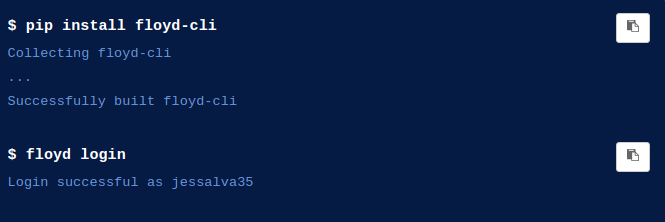
\includegraphics[width=3in]{FloydHub_partOne.png}
	    \end{center}
	    
    \begin{itemize}
    
        
	    \item floyd-cli was successfully installed on the system.
	    
	   
	\end{itemize}
     
	    \begin{center}
	        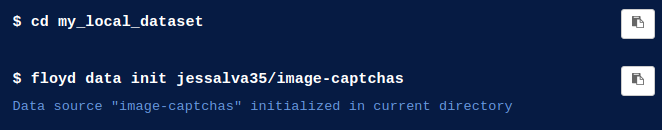
\includegraphics[width=3in]{FloydHubTwo.png}
	    \end{center}
	    
\end{frame}

\section{Next Step}
 \begin{frame}{Next Step}
 \begin{itemize}
     \item The dataset will be uploaded. 
     \item Training will be done in the cloud GPU.
     \item Once we have attained the required accuracy, we can download the weights and use them in our system.
     \item We can extract the gradients using the trained model's weights to perform attack on the dataset.
     \end{itemize}
 \end{frame}
\begin{frame}{}
  \centering  \Huge{Thank You}
\end{frame}

\end{document}
